\chapter{}

\section*{Из воспоминаний Э. И. Певзнер.}

Почти 30 лет, со дня моего рождения~-- в 1935г. и до почти 1965г., когда моей доченьке Юле исполнилось 4 года, я прожила в моем любимом, обожаемом дома на Хоромном, у Красных ворот. Этот дом был совершенно особым, со своим миром, со своими законами.

Моя мама, Тейтельбаум Мария Исааковна, вернувшись в 33 году из Бермена, где она работала в Советском Торгпредстве у наркома Литвинова, заплатила (по ее словам) <<золотой валютой>> за трехкомнатную квартиру. Впоследствии, уже перед войной, квартиры перестали считаться кооперативными, и к нам в большую комнату подселили семью~-- из двух человек~-- оба партийцы. Андрей Владимирович Мякишев и его жена~-- Макагон Александра Васильевна. С ними я прожила 25 лет, очень дружно.

Дом наш был построен в виде печатной буквы П, где перекладина была обращена во вне, а все остальное~-- семь подъездов~-- помещались внутри. В дом можно было попасть только через огромные чугунные решетчатые ворота, которые в то время не запирались, и мы, дети, любили на них кататься. После ворот шла довольно длинная арка. До войны на правой стене (от ворот) помещались большие и глубокие ящики с деревянными дверками~-- туда <<особо ответственным товарищам>> доставляли продовольственные заказы. А таких жильцов, особенно до войны, было большинство. По другую сторону арки была каморка с окном~-- сторожка, где всегда сидел дежурный лифтер.

Внутри дома был маленький, уютный дворик, в середине круглый фонтан, потом пристроили песочницу для малышей, а для больших~-- был сколочен простой деревянный стол и две скамейки-лавки по бокам.

И вот настали страшные 37--38 годы. Из 95 квартир нашего дома 60 были опустошены. Людей очень уважаемых в стране, ответственных работников забирали, как правило, по ночам. Объявляли приговор: <<10 лет без права переписки>> (что на деле означало расстрел). Состав дома переменился.

Многие, когда началась война, уехали в эвакуацию. Но в 43 году почти все, оставшиеся в живых, вернулись. В том числе и наша семья. В этом же году я пошла в школу (613-ю женскую~-- первый опыт).

Но вся моя жизнь, как и жизнь всех, проходила в доме, во дворе. Мы дружили~-- целыми поколениями, по возрасту. <<Нашего брата>> было тогда довольно много: Миша Плоткин, Лева Месежников, Боба Моргунов, Галя Столяровская (на год моложе), Рита Гиргидова и Инна Платонова (обе на год старше), сюда же примыкали Женька Займовский, Марик Миникс, а вот Юрка Верещагин, Юрка Райский и Левка Меньшиков считались как бы уже в другой компании [Немного не так. М.М.].  Мы самозабвенно играли в Молодогвардейцев.

Были еще и <<большие ребята>> (так мы их называли). К ним я~-- бойкая девчонка~-- пристраивалась каждый вечер когда они~-- Альчон Горностаев, Шурик Штейнберг и др. тайком поднимались через чердак 5-го подъезда и выходили на крышу~-- смотреть салюты. И как только я, малявка, не сверзилась тогда и не разбилась вдребезги!

Вся жизнь наша шла во дворе, у всех на виду. <<Большие ребята>>, сидя за столом во дворе, в 1947 году читали вслух только что вышедшие в издательстве <<Советсткий писатель>> <<12 стульев>> и <<Золотой теленок>>. Мы, младшие, умирали со смеху и знали их наизусть. (Кстати, потом книгу сразу же запретили~-- и до смерти Сталина она больше не издавалась.)

Главным <<книгочеем>> нашего дома считалась Леля Александровская из 3-го подъезда. Она постоянно просиживала во дворе с книгой в руках, не вынимая изо рта большой палец, который сосала. А на столе часто ставили патефон, и <<большие ребята>> кружились со своими сверстницами. Точно, как по песне Окуджавы о Леньке Королеве, но нам завидовать им было некогда.

Из досок мы устроили качели и, стоя, подлетали прямо под кроны деревьев. Почти каждый день играли в лапту, в штандер, а особенно любимой была игра в казаки-разбойники. Прятаться бегали аж на <<задний двор>>, где была помойка (никаких мусоропроводов в помине не было, все выходили с ведрами и выносили их на задний двор). Дом наш был удивителен еще и тем, что все были свои, т.е. не было никаких пришлых, никаких хулиганов.

<<Чужими>> были только два друга~-- Юлька Зайчик, двоюродный брат Женьки Займовского, да Юрка Епишин из соседнего, бандитского дома,~-- оба безнадежно влюбленные в мою подругу Инну Платонову. Инка была тихой, скромной, неразговорчиво девочкой. Отца ее посадили, мать тоже, в комнату после войны приехала какая-то Зоя, обещавшая матери воспитывать Инку. Жили они в квартире 55, прямо напротив нашей 54-й на 6-ом этаже в 4-ом подъезде. Вообще, если рассказывать только о жильцах нашего подъезда, так это~-- целый том.

Сколько себя помню, мы целые дни носились друг к другу~-- я на третий, к Бобке Моргунову, он~-- ко мне. У нас с ним была страсть к книгам, особенно в то время к научной фантастике. Ежедневно мы виделись с Галкой Столяровской и Левкой Месежниковым из 52-й квартиры, как раз под нами. С мамой Левки~-- Ией Михаиловной и Галкиной мамой~-- Бэбой Матвеевной я могла говорить обо всем, почти как с родителями. На четвертом этаже жили Рабиновичи~-- чудесная, добрейшая Елизавета Ефимовна с двумя сыновьями~-- Эмиком и Натиком. Потом, подрастая, я очень дружила с их женами~-- Таней и Валей. А Валину дочку~-- очаровательную белокурую Инночку с личиком ангелочка~-- учила игре на фортепиано моя любимая подруга Маша, когда  мы с ней были студентками иняза. Она~-- Инночка~-- почти <<последняя из Могикан>>~-- до сих пор живет в старой квартире. Чудо! Напротив них, в квартире №50 жил знаменитый Штейн~-- зам. Молотова, в ранге посла.

Помню время перед смертью Сталина~-- самый разгул антисемитизма. Я ничего не понимала, верила, дура, газетам. Встречала его, без погон, в подъезде, страшно подавленного, но, слава Богу, не посаженного. А его жена преподавала на дому вокал. И когда бы ты ни шел по подъезду, всегда раздавалось это а-а-а-а-а-а-а! Это никого не раздражало.

На 3 этаже жили Кунины~-- очень славные. А на 2 этаже~-- уникальная личность, как говорили у нас тогда, друг Ворошилова~-- Иона Каменский. Рассказывали шепотом, что на голове у него какая-то огромная штука. Была у него взрослая дочка~-- Ирка Каменская. Все называли ее Камека. Считалось, что она сверхэкзальтированная девица. Рассказывали, что папаша бьет ее смертным боем, а она выскакивала во двор, ложилась на пол, орала и считалась истеричкой, а вообще она, наверное, была несчастное создание, рано лишившееся матери.

Еще я очень хорошо помню трех молодых людей, просто трех мушкетеров, из хороших, благовоспитанных семей~-- Алика Гриневского из 1-го подъезда, Вовочку Андреева из 2-го и Сергея Дивильковского из 3-го. Мы необидно называли их (по порядку)~-- Спичка, Супчик и Кашка. Все трое потом стали знамениты: Алик~-- посол (после МГИМО), Вовочка~-- народный артист, художественный руководитель театра Ермоловой, а Сергей, закончивший МГИМО,~-- крупный дипломат.

Вообще, люди в нашем доме были замечательные. У нас жил в 6-ом подъезде ставший знаменитым детский писатель Юра Коваль. В 5-ом подъезде жили сестры Клейн~-- все с медицинским образованием. В 1-ом подъезде до сравнительно недавнего времени жила знаменитая переводчица со скандинавских языков и писательница~-- Юлиана Яхнина.

И красавицы у нас были такие~-- просто глаз не оторвать. Например, в 5-ом подъезде, сразу же после войны, проживала расфранченная дама Элеонора Борисовна Крейндлина с дочкой Лорочкой~-- принцессой с голубыми глазами и золотыми кудрями. В 7-ом подъезде жила девочка уникальной внешности: с ресницами на полметра и прекрасными карими глазами~-- Туся Еременко. К ней тяготела ставшая красоткой Анечка Вайнштейн.

Для меня, девчонки войны, вобравшей в себя всю любовь к Родине и товарищу Сталину, самое интересное время после войны было в Красном Уголке. Находился он в 5-ом подъезде, где для него отвели подвал. Там была хорошая сцена и зрительный зал. Почти ежедневно там крутили все любимые наши фильмы тех лет~-- и все их мы смотрели десятки раз, и все бесплатно.

Работали там и кружки: хоровой, драматический, танцевальный. Я, конечно, была их активным членом. Возглавляла всю самодеятельность некая Ангелина Сергеевна Спартак~-- крепкая, полная, невысокого роста блондинка с крашенными перекисью волосами. Ее подселили в маленькую комнату квартиры Моргуновых в нашем подъезде. Она ставила с нами пьесы, разучивала песни и стихи.

Потом были концерты. Приходили наши мамы и бабушки. Мы были герои дня. Особенно отличился малыш~-- Владик Каплун, брат Кати из 1-го подъезда. Он прочел стишок:

\nepage

{\itshape

    Вот какой коташка,
    
    Круглая мордашка.
    
    И на каждой лапке
    
    Коготки-царапки.
    
    Все ему игрушка:
    
    Кубик и катушка.
    
    Котик, словно мячик,
    
    По квартире скачет. Мяу!
    
}

\indent

С тех пор Владик свое имя потерял. Его стали все~-- поголовно~-- называть только Коташка. Вообще, жизнь во дворе у нас била ключом. Сами мы домой не уходили~-- приходилось загонять. Каждый вечер мой папа, встав на подоконник в маленькой комнате, на 6-ом этаже, окнами во двор, кричал одно и то же: <<Элуша, домой!>> И только тогда приходилось прерывать игру и ехать на старом лифте наверх. Как было весело во дворе, как захватывающе интересно! Ведь родители наши работали целые дни, а тут мы были все вместе.

Когда я, уже став взрослой, катала по двору страшную зеленую коляску, где лежала моя новорожденная дочурка, я еще и не предполагала, что если бы не чудесный детский доктор из 2-го подъезда~-- Эсфирь Яковлевна Бару, то моя крошка запросто могла бы погибнуть (у ребенка началась диспепсия). Э. Я. строго-настрого приказала мне ежедневно носить к ней домой пеленку с детскими какашечками. По цвету и запаху она определяла, что делать дальше, как лечить. Я всю жизнь молюсь и вспоминаю Э. Я.

Были у нас во дворе и страшные вещи: погиб, долго болея, мальчик из 2-го подъезда, Боренька Пенько. Помню его бедную тихую маму, маленькую, рассказывающую нам, что у Бореньки была саркома. О такой болезни я тогда и слыхом не слыхал. А когда утонул мой детский друг Левушка Месежников, это было просто первой, очень страшной моей личной трагедией. Ведь я и сама осталась жива просто чудом~-- и если бы не было коммунальных квартир~-- просто погибла бы, так как у меня в 7 лет был острейший приступ аппендицита, а вызванная из районной поликлиники молодая врачиха, сразу после института, его не распознала. И только соседка наша, тетя Шура, отвела мамину руку с кипятком~-- налить грелочку~-- предположив: <<А вдруг у Элки аппендицит>>. А генерал Иванцов из 5-го подъезда, чья машина стояла на счастье во дворе, тут же приказал своему шоферу везти меня в больницу, аж на край света в то время~-- в Измайлово~-- где был военный госпиталь!

Я была настоящей девчонкой своего времени, своего двора. Сколько часов я проводила в сторожке беседуя с моей любимой Фридой Абрамовной, мамой Марика Миникса, или потом, поверяя Тане, работающей у семье Медниковых, свои первые любовные секреты.

Как хорошо, что дом наш существует, хотя многих уже нет: ушли из жизни, переехали. Но в нем живут такие люди, как удивительная Танечка Меньшикова, член <<Мемориала>> и Совета Ветеранов микрорайона, поддерживающая историю дома, помогающая всем и хранящая идеалы прежних лет. Она~-- светлая, добрая луша нашего дома, вечно юная и несгибаемая.

Я через всю  жизнь пронесла любовь к моему первому в жизни дому, где мы все жили, как одна дружная семья, несмотря на все тяжести и страдания тех страшных лет.

\indent

\begin{figure}[h!]
    \begin{minipage}[t]{70mm}
    \thisfloatsetup{capbesideposition=right}
    \hspace{1pt}\fcapside[\FBwidth]{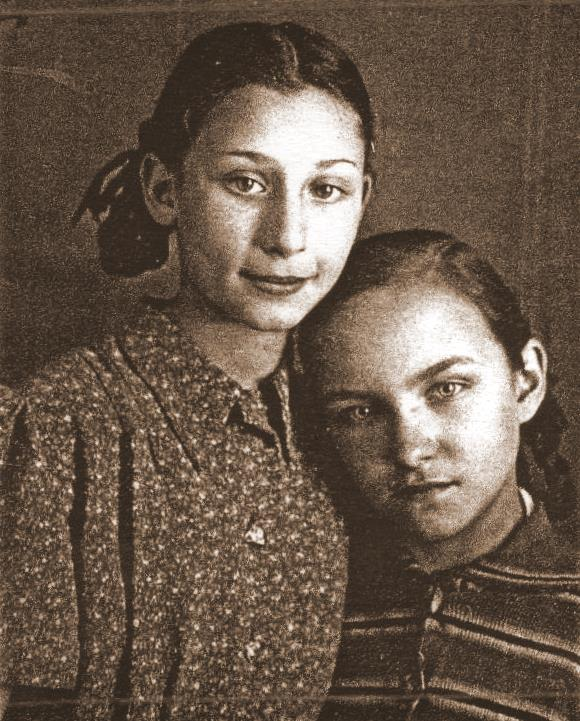
\includegraphics[width=23mm]{inc/94/2}}{    \caption{Элла Певзнер с \\Инной Платоновой. }}
    \end{minipage}
\end{figure}

\indent

\begin{figure}[h!]
    \begin{minipage}[t]{70mm}
    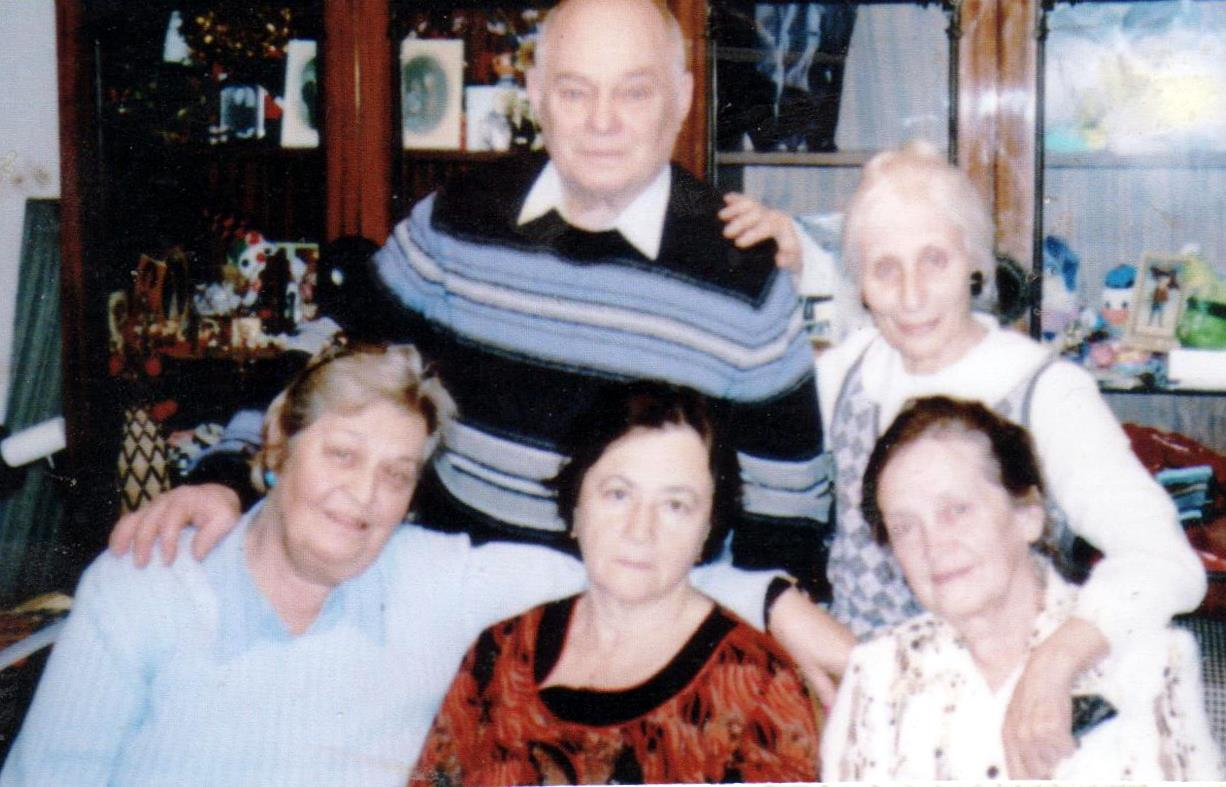
\includegraphics[width=70mm]{inc/94/1}
    \footnotesize{\textit{Э. И.. Певзнер с М. М. Плоткиным и женами М. М. Плоткина, М. В. Миникса и \\ Б. И. Моргунова.}}
    \end{minipage}
\end{figure}
